\documentclass{article}
\usepackage{graphicx}
\usepackage{wrapfig}
\usepackage[hmargin=3.5cm,vmargin=3.5cm]{geometry}
\begin{document}

\title{TI2800 Contextproject - Cultural Heritage \\ Requirements Analysis}
\author{Sjoerd van Bekhoven \\ Tim Eversdijk \\ Herman Banken \\ Rutger Plak \and 4014774 \\ 4005562 \\ 4078624 \\ 1358375}
\maketitle

\section{Doelgroep}
Het systeem zal voorzien in informatie over en verbanden tussen monumenten, maar zal ook informatie geven over wat er om de monumenten heen vindbaar is. Hierbij kan gedacht worden aan caf\'es, restaurants of openbare voorzieningen. Daarnaast is er de mogelijkheid om een route uit te stippelen. De beoogde doelgroep bestaat dus toeristen die bijvoorbeeld:
\begin{itemize}
		\item{een intellectueel dagje uit in een bepaalde stad willen plannen.}
		\item{een weekend door Nederland willen toeren langs verschillende monumenten.}
		\item{informatie over een bepaald monument willen opzoeken.}
		\item{willen opzoeken in welke stad de interessantste monumenten te bezoeken zijn.}
		\item{een monument gaan bezoeken en willen weten waar ze daarna wat kunnen eten of drinken.}
		\item{een monument hebben bezocht en graag inspiratie willen opdoen over andere gerelateerde of soortgelijke monumenten.}
\end{itemize}
Volgens de World Tourism Organization is een toerist iemand "die reist naar plaatsen buiten zijn/haar gebruikelijk milieu, die niet meer dan \'e\'en jaar voor vrije tijd, zaken en andere doeleinden blijft en die niet beloond wordt voor zijn/haar activiteit ter plaatse".\footnote{http://pub.unwto.org/WebRoot/Store/Shops/Infoshop/Products/1034/1034-1.pdf, World Tourism Organization. 1995. p. 14. Retrieved 2009-03-26} \\
Het systeem zal voornamelijk worden toegespitst op toeristen, maar zal ook voor kenners, wetenschappers, scholen, studenten e.d. een interessante informatiebron worden. Naast toeristen, zullen ook zij het voor hen relevante deel van het systeem kunnen gebruiken.
\clearpage
\section{Systeem requirements}
De vereisten van het te maken systeem verdelen we onder in verschillende kopjes.
\begin{enumerate}
	
	\item{\textbf{Requirements Gebruiker}}
	\begin{enumerate}
		\item{\textbf{Gebruiksomgeving:}}		
		Het systeem zal gebruikt worden in de toeristische sector. Toeristen kunnen via de webinterface zoeken naar een monument om te bezoeken. Het systeem zal dus in de huiselijke sfeer worden gebruikt, maar ook mobiel, wanneer de toerist bij het monument aankomt en de achtergrond informatie nog bij de hand wil hebben. Ook onderweg zal hij het systeem willen gebruiken.
		\item{\textbf{Missie profiel of scenario:}} How will the system accomplish its mission objective? 
		
		Het systeem is opgedeeld in een webinterface en een back-end. De back-end verzamelt en berekent alle data die de webinterface kan gebruiken. Deze back-end gebruikt een dataset met alle monumenten in het Rijksmonumenten register en bij behorende afbeeldingen uit Wikimedia Commons. Daarnaast verzamelt deze extra input gegenereerd door gebruikers zoals reacties op afbeeldingen en pagina\'s. Op deze manier weet de back-end te bepalen of monumenten relevant zijn of niet. 
		
		\item{\textbf{Prestaties en bijbehorende parameters:}}
		
		De beschikbare data is een kritische systeem parameter omdat het van de data afhangt wat het systeem de gebruiker kan laten zien. Wanneer het systeem de gebruiker geen relevante informatie kan geven dan is de missie gefaald.
		
		\item{\textbf{Interface:}}
		
		De webinterface bestaat uit diverse onderdelen. Allereerst is er een kaart met daarop de gefilterde monumenten. Deze kaart is te gebruiken om snel een geografische selectie te maken van de monumenten. Er is een filter-component waar gebruikers aan de hand van gegeven labels danwel berekende selectiecriteria monumenten kunnen filteren. 
		
		De pagina met kaart bevat ook een lijst met aanbevolen monumenten op basis van eerder bekeken monumenten gefilterd op relevantie en beoordeling door andere gebruikers. Deze kunnen worden aangeklikt zodat de gebruiker ze kan bekijken.
		
		Het detailoverzicht van een monument bevat informatie over het monument zelf. De toerist kan zich zo vast verdiepen in het monument. Daarnaast bevat deze pagina aggregated data van weersinformatie, hotelboeking-sites, etc. Onderaan vindt de toerist aanbevolen monumenten aan de hand van het getoonde monument, user-input, eerder bekeken monumenten en andere rankings-criteria.
		
		\item{\textbf{Effectiviteit:}}
		
		Het systeem moet direct al interessante monumenten kunnen tonen. Gebruikers weten niet waar ze op moeten zoeken maar moeten wel direct vastgehouden worden, dus ook als ze niet naar iets specifieks op zoek zijn. Ze moeten binnen enkele minuten iets kunnen uitkiezen. Het systeem moet de gebruiker dus heel snel kunnen informeren.
	\end{enumerate}
	\item{\textbf{Systeem architectuur}} 
We hebben een java backend draaien waar verschillende features zullen worden bepaald en berekend. Er zal een sql server worden gebruikt om user data en monumenten informatie in op te slaan en op te vragen. Vervolgens zal de front-end web based zijn en draaien op een php server.
	
\end{enumerate}
\section{Mogelijke valkuilen}
\begin{itemize}
\item Cold start: in het begin is er nog nauwelijks user data beschikbaar behalve die van Flickr. De recommendations zijn daarom nog nauwelijks gebaseerd op user-input.
\item Long tail: veel ongebruikte data. Nooit bekeken monumenten worden ook later niet meer gevonden.
\end{itemize}
\section{Meetbare doelen}
\begin{itemize}
\item Het is een goal om een zo hoog mogelijk percentage relevante / niet relevante fotos te vinden/weergeven d.m.v beeld en tag informatie bij verschillende criteria zoals:
\begin{itemize}
\item dag / nacht
\item indoor / outdoor
\item gebouw / geen gebouw
\end{itemize}

\end{itemize}
\section{Prototypes}
Om een beeld te geven van hoe het systeem eruit komt te zien, zijn deze beelden gemaakt in \emph{Balsamiq}. 

Wanneer de gebruiker het systeem opent ziet hij het overzichtsscherm zoals te zien in figuur 1. Aan de hand van de verschillende selectiecriteria aan de rechterkant van het scherm kan de gebruiker de selectie monumenten zichtbaar op de kaart beperken.
\begin{figure}[htp]
  \centering
  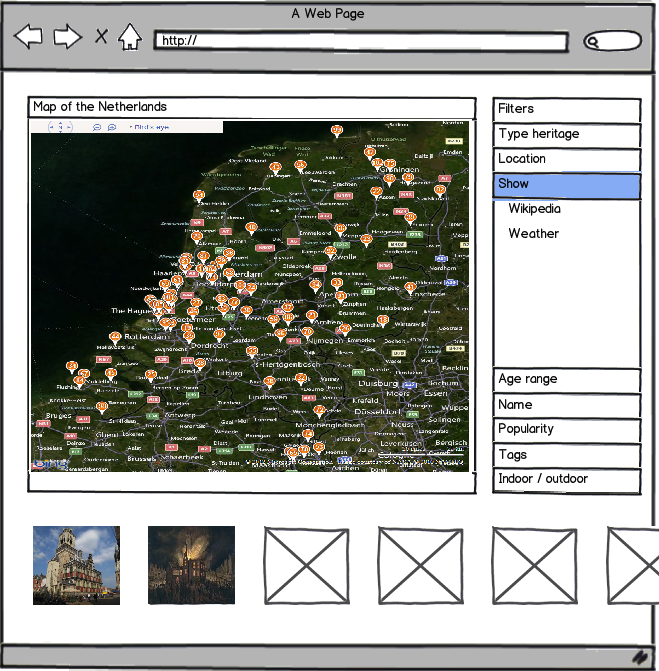
\includegraphics[width=3in]{user-story-overview.png}
  \caption[Het overzichtsscherm]%
  {De kaart van Nederland, met rechts ervan selectiecriteria aan de hand waarvan de monumenten op de kaart worden getoond of verborgen.}
\end{figure}

Heeft de gebruiker een monument geselecteerd, dan wordt de detailpagina, als te zien in figuur 2, getoond. 
\begin{figure}[htp]
  \centering
  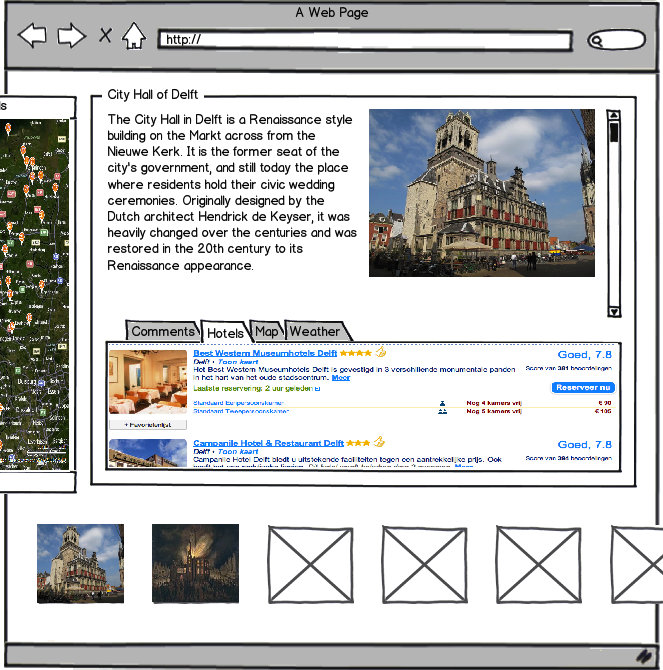
\includegraphics[width=3in]{user-story-detail.png}
  \caption[Voorbeeld van een detailpagina van een monument]%
  {In dit scherm zijn de details te zien van een gekozen monument, met de besproken opties.}
\end{figure}

\section{Software requirements specification}
We onderscheiden de \emph{serverside} van de \emph{clientside}.
De systeemvereisten voor de server zijn:
\begin{itemize}
	\item{PHP $>= 5.2.x$}
	\item{MySQL $>= 7.x$}
	\item{JAVA $>= 1.5$}
	\item{Apache $>= 2.3$}
\end{itemize}
De systeemvereisten voor de client zijn:
\begin{itemize}
	\item{Webbrowser met V8 Javascript Engine}
\end{itemize}
\end{document}